\section{Valuation}
Valuation of options has been a great area of research, starting with Black-Scholes derivatives pricing and building upon it.
    Relevant for accounting statements and tax returns - FASB has changed valuation practices several times to ensure harmonization
    shape of valuation function → executive's exposure to risk and incentives
    valuation and hedge ratio/delta provide approximation of the incentive of option (which remain however limited and dependent on the full comp package!)

    The difference between the objective and subjective value originates in the non-transferability of the options to different holders and the restriction on short selling of the firm’s stocks as a hedging strategy in the portfolio.

    We compute the cost to the employer under the risk neutral framework and the executive value under the utility maximizing framework. 

    %Objective value: use binomial model mainly
    %Subjective value: certainty equivalence procedure

    %Note that in the below we assume that the stock price follows a simple geometric Brownian motion, not influenced by the agents' actions, which is standard in the literature. A different approach could be accounting for it, at least in the executive valuation part, which could be a sensible thing to do. Anyhow, our approach can be seen as a lower bound approximation for such revised executive value (with effort = 0 and no additional executive-induced volatility).


\subsection{Valuation models} 

\subsubsection*{Black-Scholes}
    The Black-Scholes model, developed by Fischer Black and Myron Scholes in the early 1970s (\cite{black1973pricing}), is a well-known mathematical framework used in finance to determine the theoretical value of European-style options. A more detailed overview of the model is out of our scope and can be easily found online. We will just limit ourselves to the minimum requirements and intuition to be able to use the Black-Scholes model in computing the time-value of our ESOs later.
    
    The assumptions are quite standard, so we simply take them from \cite{wiki:blackscholes}:

    \begin{assumption}
        \label{ass:bs_1}
        The rate of return on the riskless asset is constant and denoted as risk-free interest rate $r$.
    \end{assumption}
    

    \begin{assumption}
        \label{ass: bs_2}
        The instantaneous log return of the stock price is an infinitesimal random walk with drift: the stock price follows a geometric Brownian motion, and it is assumed that the drift and volatility of the motion are constant.
    \end{assumption}

    \begin{assumption}
        \label{ass:bs_3}
        The stock does not pay any dividends.
    \end{assumption}

    \begin{assumption}
        \label{ass:bs_4}
        The market is arbitrage-free.
    \end{assumption}

    \begin{assumption}
        \label{ass:bs_5}
        It is possible to borrow and lend any amount (even fractional) of cash at the riskless rate.
    \end{assumption}

    \begin{assumption}
        \label{ass:bs_6}
        It is possible to buy and sell any amount (even fractional) of the stock.
    \end{assumption}
    
    \begin{assumption}
        \label{ass:bs_7}
        There are no transaction fees.
    \end{assumption}
    
    Note that the first three assumptions are about the underlying asset while the last four are about the market. Moreover, assumption \ref*{ass:bs_6} assumes the possibility of short-selling and free trade of firm's stock, which in the case of ESOs is usually not feasible as it comes with limitations. However, the Black-Scholes model provides nevertheless a good approximation and suffices for our (limited) use. Note however that not all of these assumptions are strictly necessary: extensions of this basic model are able to account for dynamic interest rates, transaction costs and taxes, and dividend payout.  

    Under these assumptions, \cite{black1973pricing} showed that it is possible to create a hedged position (i.e., a long position in the underlying stock and a long position in the option) whose value is independent of the price of the underlying. This dynamic hedging strategy leads to a partial differential equation governing the price of the option, whose solution is given by the Black-Scholes formula.

    However, despite its mathematical rigor and closed-form solution, as well as computational efficiency, the Black-Scholes can only be used with European options (options exercisable only at maturity). Therefore, since we are dealing with American ESOs, we need to resort to a different valuation methodology: binomial model.

\subsubsection*{Lattice tree methods)} 
\textbf{Binomial model}
The binomial model was first proposed by William Sharpe in the 1978 (\cite{sharpe1978investments}) and later formalized by Cox, Ross and Rubinstein (CRR) in 1979 (\cite{cox1979option}). It uses a lattice-based approach to model the price of the underlying stock price. We employ it to value our executive stock options, since they are, as we saw before, American options.\footnote{Recall that Black-Scholes can be used only with European options, i.e., options exercisable only at maturity. Nevertheless, Black-Scholes valuation provides a lower-bound to the value of American options. Indeed, giving the holder the possibility to exercise before maturity also cannot be worse for her, because she can always simply hold the option up to maturity and then deciding, mimicking thus a European option.}
Similarly to Monte Carlo simulations and finite difference methods, the binomial options pricing model does not yield a closed-form solution, but works quite well with sufficiently high number $n$ of time steps, i.e., with a sufficiently discretized grid (i.e., a small $\Delta t$). Clearly, for European options, as $\Delta t \rightarrow 0$, the binomial model approaches the Black-Scholes value.

We need assumptions \ref*{ass:bs_1}, \ref*{ass:bs_3}, \ref*{ass:bs_4}, \ref*{ass:bs_7} from Black-Scholes, and in addition we pose two additional assumptions:

\begin{assumption}
    \label{ass:bin_8}
    Time is divided into discrete periods.
\end{assumption}

\begin{assumption}
    \label{ass:bin_9}
    At any time step, the underlying's price can only move one of two ways: either up or down.
\end{assumption}

The intuition behind the model is quite simple. We discretize the evolution of the underlying stock price by building a binomial lattice (tree), for a given number of steps between the issue of the option and its maturity. Each node represents thus a possible price of the underlying stock. From each node, the stock price can either go up ($u$) or down ($d$). The key assumption is thus that the stock moves only in either one of these two directions. Therefore, the generic value of the stock at step $t$ with $k$ upward movements and $t-k$ downward movements is $S_t = S_0 u^k d^{t-k}$, where $S_0$ is the initial stock price at $t=0$. Figure \ref*{fig:bin_tree} provides a graphical representation of the first two levels of the stock price tree. 

\vspace*{3pt}
\begin{figure}[!h]
\vspace*{10pt}
\centering
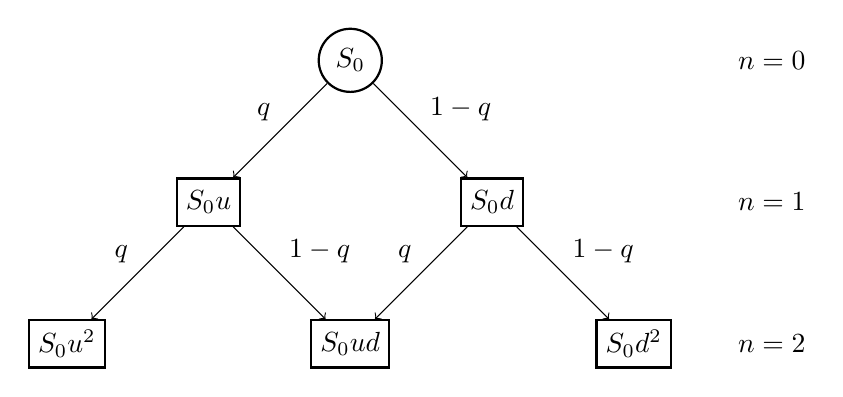
\begin{tikzpicture}[
    roundnode/.style={circle, draw=black, thick, minimum size=6mm},
    squarednode/.style={rectangle, draw=black, thick, minimum size=6mm},
    scale=1.2
  ]
  
  %Nodes
  \node[roundnode] at (0,0) (A) {$S_0$};
  \node[squarednode] at (-1.5,-1.5) (B) {$S_0 u$};
  \node[squarednode] at (1.5,-1.5) (C) {$S_0 d$};
  \node[squarednode] at (-3,-3) (D) {$S_0 u^2$};
  \node[squarednode] at (0,-3) (E) {$S_0 ud$};
  \node[squarednode] at (3,-3) (F) {$S_0 d^2$};  
  
  %Lines
  \draw[->] (A) -- (B) node[midway,above left] {$q$};
  \draw[->] (A) -- (C) node[midway,above right] {$1-q$};
  \draw[->] (B) -- (D) node[midway,above left] {$q$};
  \draw[->] (B) -- (E) node[midway,above right] {$1-q$};
  \draw[->] (C) -- (E) node[midway,above left] {$q$};
  \draw[->] (C) -- (F) node[midway,above right] {$1-q$};
  
  %Labels
  \node[right] at (4,0) {$n=0$};
  \node[right] at (4,-1.5) {$n=1$};
  \node[right] at (4,-3) {$n=2$};

\end{tikzpicture}
\caption{Representation of the binomial tree with n=2} 
\label{fig:bin_tree}
\end{figure}
\newpage  %%-> FIX q/1-q location on arrows

We can divide the procedure in three main steps: (i) build the stock tree, (ii) calculate the option value at each terminal node, (iii) go backwards and decide at each node whether it is optimal to exercise or keep the option.

We use the original CRR method and set $u = e^{\sigma \sqrt{\Delta t}}$ and $d = e^{-\sigma \sqrt{\Delta t}}=\frac{1}{u}$, which are the multiplicative factors if the stock price goes up or down, respectively. Note that the price multipliers $u$ and $d$ depend thus only on volatility of the underlying and time step $\Delta t$ and not on the drift.\footnote{This is the reason for which the probability of going up is usually higher in this model, to compensate for the missing account of the drift component} Therefore, the value of the stock when it goes up or down depends also on its underlying volatility. Moreover, the condition $d = \frac{1}{u}$ ensures that the tree is recombinant, meaning that what matters is the number of ups and downs, not their order. This means that if the stock price moves up and then down, the stock price will be the same as if it instead moved first down and then up. This is convenient also because it allows the tree representation of the underlying stock price, ensuring that all the nodes are nicely connected, and it fastens the calculation of the option price (indeed, note that in this way the number of total nodes is reduced). 

In the second step, we simply compute the option value at expiration, i.e., its intrinsic value, which in our case is $\max \{0, S_T - K \}$ since we have a call option.

For the third step, we need to introduce the risk-neutral probability $q = \frac{e^{-r \Delta t} - d}{u-d}$ which assesses how likely is that the stock price goes up during each period in a risk-neutral world. \footnote{This choice of $q$ allows for the related binomial distribution to simulate the geometric Brownian motion of the underlying stock, with parameters $r$ and $\sigma$.} In this world, today's fair price of the option is the expected value of its future payoff discounted by the risk-free rate. Therefore, the expected value at time $t$ is calculated using the option values from the subsequent two nodes at $t+1$, weighted by their respective probabilities - $q$ as the probability of an upward move of the underlying stock, $1-q$ of a downward move. This value is then discounted using $r$ and represents the \textit{binomial value} of the option at a given node. 
Given $q$, we can then proceed with our backwards algorithm. We start at each pre-terminal node and evaluate whether it is optimal to exercise (with payoff the stock price at the node minus the strike price) or to not exercise (with payoff the binomial value at the node). We continue this process iteratively going backwards until when the option is vested. When the option is not vested anymore, the holder cannot exercise it and so the value of the option will simply be the binomial value, at that node and all the previous ones.
The value of the option at the initial node, obtained with this backwards procedure, is the value of the ESO we obtain using the binomial model.
This is the traditional backwards approach; however, we will modify slightly the decision function in the last step to account for the tendency of early exercise.

\textbf{Trinomial model}
The trinomial option pricing model was  first developed by Phelim Boyle in 1986 as an extension of the binomial model. Conceptually the two models are the same: here we are only allowing for the stock to have a third path, the middle path, whereby it does not go down nor up but remains stable. Therefore, the differences from the binomial model are very few. We replace assumption \ref*{ass:bin_9} with the following:
\begin{assumption}
    \label{ass:trin_10}
    At any time step, the underlying's price can only move one of three ways: either up, down, or remain stable.
\end{assumption}
As before, $u = e^{\sigma \sqrt{\Delta t}}$, $d = e^{-\sigma \sqrt{\Delta t}}=\frac{1}{u}$, and now $m=1$. Moreover, we need to change the risk-neutral probabilities (before we had two, now three), which become slightly more complicated:\footnote{Recall that we do not consider dividend yields on our stock, hence the formulas are slightly easier than usually presented.}
$$ q_u = \Biggl(\frac{e^{r \Delta t / 2} - e^{-\sigma \sqrt{\Delta t / 2}}}{e^{\sigma \sqrt{\Delta t / 2}} - e^{-\sigma \sqrt{\Delta t / 2}}}\Biggr)^2 $$
$$ q_d = \Biggl(\frac{e^{\sigma \sqrt{\Delta t / 2}} - e^{r \Delta t / 2}}{e^{\sigma \sqrt{\Delta t / 2}} - e^{-\sigma \sqrt{\Delta t / 2}}}\Biggr)^2 $$
$$ q_m = 1 - (p_u + p_d) $$

Therefore, the idea of the procedure is the same: we compute the stock price tree and then proceed backwards to determine the optimal decision at each node. The difference now is that the option at each non-terminal node is computed based on three later nodes - instead of two - and their relative probabilities.
The trinomial model produces more accurate results compared to the binomial model when using fewer time steps, but the binomial model is usually preferred due to its faster implementation.

\subsection{Firm cost} 
%Objective value

We compute the cost of the two options to the firm using the classical valuation standards for ESOs: a simple binomial model for the RN option, and a modified binomial model that accounts for the recovered time premium for the R option.
Recall indeed that the theoretical value of an option at any time $t$ is given by (i) the intrinsic value ($S_t - K$) and (ii) the time premium, i.e., the remaining value forfeited at exercise, as the option could have appreciated in the remaining lifetime. 
We employ the \cite{cox1979option} initial binomial tree approach; however, we account for "deterministic" early exercise introducing a threshold above which the holder will exercise, i.e., always exercise if $S_t \ge Km$ for some multiple m (\dots).

We now comment the relevant code used - the full code can be found in the appendix.

\subsubsection{RN option}
The function rn\_eso is defined as \verb|rn_eso(S0,K,T,v,r,N,sigma,m)| and takes the following parameters as input:
\begin{itemize}
    \item $S$: spot price of the underlying firm stock
    \item $K$: strike price of the option. In our case, we always set it equal to S \footnote{some propose to set it slightly higher ...}
    \item $T$: time to maturity (in years)
    \item $v$: vesting period of the option (in years)
    \item $r$: risk-free interest rate
    \item $N$: height of the tree
    \item $sigma$: volatility of the underlying firm stock
    \item $m$: exercise multiple
\end{itemize}

    
We follow the binomial model procedure illustrated before: we first construct the stock price tree and then we compute the option's value backwards. As mentioned above, we change slightly the decision function at each node, using the multiple technique proposed by \cite{hull2002determining}. Therefore, we model early exercise as taking
place whenever stock price reaches a certain multiple - from here the name - of the strike price.
At each step, the relevant decision is the following: if the option is either not vested or is vested but is not above the threshold for early exercise, the value at the node is the binomial value. Otherwise, if it is vested and above the threshold for early exercise, the value at the node is the exercise value. This procedure is illustrated in snippet \ref*{fig:val_rn}.

\begin{figure}[H]
    \begin{lstlisting}[breaklines, basicstyle=\ttfamily\small]
    if not vested: 
        C[j] = disc * (q*C_up + (1-q)*C_down)
    elif vested & (S>=K*m):            
        C[j] = S - K
    elif vested & (S<K*m):
        C[j] = disc * (q*C_up + (1-q)*C_down)
    \end{lstlisting}
 \label{fig:val_rn}
\end{figure}

\subsubsection{R option}
We define the function r\_eso as \verb|r_eso(S0,K,T,v,r,N,sigma,m,alpha,gamma)|.
    


We use the same parameters as above, with the addition of:
\begin{itemize}
    \item $\alpha$: amount of option that gets converted to stock at exercise
    \item $\gamma$: \textit{risk premium} granted in terms of new RN option 
\end{itemize}

The valuation here is trickier because the payoff at exercise is not anymore only the difference between the stock price and the strike price, but also the time value that gets recouped with the issue of the new option. It is hence clear that, holding the same parameters, the cost of rn\_eso is a lower bound for r\_eso. We follow the procedure proposed by \cite{huang2013dynamic} in snippet \ref*{fig:val_r_gamma0}. The difference from above is that, when the option is vested and above the threshold for (early) exercise, the payoff is not anymore given only by the intrinsic value but also by a portion of its time value, computed as the Black-Scholes cost minus the intrinisc value, multiplied by the percentage that gets recouped. 

\begin{figure}[H]
    \begin{lstlisting}[breaklines, basicstyle=\ttfamily\small]
    if not vested:                
        C[j] = disc * (q*C_up + (1-q)*C_down)
    elif vested & (S >= K*m): 
        C[j] = (S - K) + 
                (1-alpha)*(black_scholes(S,K,T,r,sigma)-(S-K))
    elif vested & (S < K*m):
        C[j] = disc * (q*C_up + (1-q)*C_down)
    \end{lstlisting}
    \caption{Valuation of RN option with $\gamma=0$}
    \label{fig:val_r_gamma0}
\end{figure}

 We run the simulation using their parameters (S=30, K=30, T=10, v=3, r=0.05, N=1, sigma=0.3, m=2) and obtain the following results: \$13.66 for RN, \$14.55 for R. Therefore, the cost of the RN option is the same as the one they find, while the cost of the R option is higher than the one they find (\$14.14). It is unclear where the difference comes from; it could simply be a difference in the choice of the number of time steps per year parametrized by N, which they do not present explicitly. Nevertheless, running the binomial model with N=1 is too low, as table \ref*{tab:diff_n} shows. Indeed, this means allowing the stock to have only one movement per year, which is quite restrictive. The results from table \ref*{tab:diff_n} suggest thus that it is safer to run the simulations with at least N=500.
 %We will do it with N=1000

 \vspace*{10pt}
\begin{table}[h]
    \centering
    \begin{tabular}{|l|c|c|c|}
       
        \hline
        \textbf{N} & \textbf{RN (\$)} & \textbf{R (\$)} & \textbf{R-RN (\$)}\\
        \hline
        1 & 13.66 & 14.55 & 0.89 \\
        \hline
        10 & 12.98 & 14.12 & 1.14 \\
        \hline
        50 & 12.79 & 14.00 & 1.21 \\
        \hline
        100 & 12.79 & 14.00 & 1.21 \\
        \hline
        365 & 12.72 & 13.95 & 1.23 \\
        \hline
        500 & 12.66 & 13.91 & 1.25 \\
        \hline
        1000 & 12.69 & 13.93 & 1.24 \\
        \hline
    \end{tabular}
    \caption{Difference in values of RN and R by changing the number of steps per year $N$}
    \label{tab:diff_n}
\end{table}

However, this valuation is incomplete, because we are not considering the role played by $\gamma$. In their paper, \cite{huang2013dynamic} show only one example, where 75\% of the option gets exercised and another 25\% (i.e., 100\% - 75\%) gets "reloaded". Therefore, it is unclear how they would consider a strictly positive risk premium $\gamma > 0$. 
We propose a similar approach which builds on their original idea. Note that the value of adding $\gamma$ is two-fold: first, as a proper exercise compensation since the executive gets stock and options worth $(1+\gamma)$ the number of options she previously held, and second as time value recovered. Therefore, we propose the valuation methodology in snippet \ref*{fig:val_r} for our R option which embeds this double edge provided by $\gamma$: \verb|1+gamma*(S - K)| captures the first, \verb|(1-alpha+gamma)*(black_scholes(S,K,T,r,sigma)-(S-K))| the second.
Clearly, this methodology equals the previous when $\gamma = 0$. Therefore, it can be seen as an extension of \ref*{fig:val_r_gamma0}.

\begin{figure}
    \begin{lstlisting}[breaklines, basicstyle=\ttfamily\small] 
    if not vested:                         
        C[j] = disc * (q*C_up + (1-q)*C_down)
    elif vested & (S >= K*m):                
        C[j] =  (1+gamma)*(S - K) + 
                (1-alpha+gamma)*(black_scholes(S,K,T,r,sigma)-(S-K))
    elif vested & (S < K*m):  
        C[j] = disc * (q*C_up + (1-q)*C_down)
    \end{lstlisting}
    \caption{Valuation of RN option}
    \label{fig:val_r}
\end{figure}


%=> Simulate also with trinomial model

\subsection{Executive value}
%-> Subjective value to different employees

%Build up on previous code
%%% Can re-use the stock price movements (both binomial and trinomial ways)
%%% Calculate at each node the utility from max{exercise, do NOT exercise}
%%%%%% -> find the utility value at initial node through recursion
%%% Using the inverse of the utility function, find the cash level that yields the same utility

%%% NOTE that our methodology is different from simply taking the value of the option computed before at the initial node and plugging it in.

We now turn to the subjective value of the option to the risk-averse executive, that we compute using the trinomial model under a utility maximization framework. In our setting, the executive is interested in maximizing its expected utility at time $t=0$; therefore, she will take a forward-looking perspective at the possible stock price grid and, by backwards induction starting from the terminal nodes, she will compute the utility she can expect given the initial parameters. This will then be translated in the amount of cash compensation she would require to give up her options, which results therefore in a certainty equivalence in continuous time. 

We build on the model proposed by \cite{lau2005valuation} that computes the value of an option with multiple reloads and fixed expiry date using a trinomial tree under the framework of maximizing the expected utility value of the terminal wealth, where the risk aversion factor is embedded in the coefficient and choice of the utility function. However, differently from them, our R option can be reloaded only once, which allows us to simplify the algorithm. For the RN option, the procedure will be even simpler. The key in both cases is that, at each non-terminal node, the executive is maximizing her utility by deciding whether to exercise or continue (hold), and this will be done as before by dynamic programming starting from the terminal nodes.
To be more precise, \cite{lau2005valuation} construct the numerical approximation extending the trinomial model via the forward shooting approach, which basically consists in augmenting the information at each node with a vector of auxiliary variables and modeling the function that describes how the vector evolves from one node to the following. We do not need such formal specification as our model is simpler than theirs; we will instead compute the non-firm related wealth available at each node using the appropriate formula rather than computing it when building the stock price tree. This approach is sensible as it is simpler yet computationally the same.

We use the same parameters from above for the two options. In addition, we need to add the following: 
\begin{itemize}
    \item $rho: $ coefficient of relative risk aversion
    \item $c: $ non-firm related initial wealth, that grows continuously at the risk-free rate $r$
    \item $n_s: $ number of stocks initially held by the executive
    \item $n_o: $ number of options initially held by the executive
\end{itemize}
Note that, at each time step $t$, the value of the non-firm related wealth $c_t$ is computed as $c_t = c \bigl(1+\frac{r}{N}\bigr)^{t}$, where $N$ is the number of time steps in a given year and $r$ the annual risk-free rate. 


As mentioned before, we want to find $E_c$ such that 
$$U(\rho, n_s, n_o, c) = U(\rho, n_S, 0, c + E_c) $$
where we included only the most relevant parameters entering the executive's utility function. Therefore, the external wealth of the executive becomes relevant now, both in terms of absolute wealth and portfolio composition (i.e., percentage of total wealth held in firm stocks). As we will see later, it is relevant because the utility function is not separable, hence our results will be sensible to the initial values we will choose.

Recall that we defined the executive's utility of wealth with the power utility function, that is, 
$$u(w, \rho) = \frac{w^{1-\rho}}{1-\rho}$$
with $\rho = 1 - \gamma $ being the (constant) coefficient of relative risk aversion. 
The inverse utility is given by 
$$w(u, \rho) = \Bigl(u(1-\rho)\Bigr)^{\frac{1}{1-\rho}}$$
We use these two formulas to define the functions \verb|u(w, rho)| and \\
\verb|u_minus(u, rho)| that return $u$ and $w$, respectively. We will use them to compute the exercise value at each node and deriving then the certainty equivalent.

%The former is the utility function in every state. Note that the function is monotonically increasing in $W$, hence also its inverse is strictly increasing, and so is the certainty equivalent. In other words, 
%The utility function is used for two purposes: deciding whether to exercise or not at each node, and deriving the certainty equivalent at time 0.

Note that we follow the approach used in the literature and assume that only block exercise is possible  to simplify our algorithm. A detailed analysis of separate exercises would be quite complex and computationally intensive. Moreover, we do not discount executive's utility from one time period to the following; in this sense, the estimates we are providing can be considered as an upper bound of the executive value.
Finally, a possible modification of the algorithm would be to embed also here an exercise multiple mechanism, that we could make dependent on the risk aversion coefficient of the executive.\footnote{For example, we could set $\frac{m}{1+\rho}$ as the threshold for early exercise for some fixed $m$, so that it would be lower for more risk averse holders. In other words, more risk averse executives would exercise earlier, which is consistent with the empirical findings.} However, we do not explore this venue here.
We will now outline briefly the main components of our algorithm, as done before.

\subsubsection{RN option}
We define the function \verb|CE_rn_trinomial(S0,K,T,v,r,N,sigma,rho, n_s,n_o,c)| to compute the executive value of the RN option. At each node, the exercise utility is computed considering the total wealth at the node, which is the sum of the non-firm related wealth $c$ invested at the risk-free rate $r$, the stock value, and the option value. Figure \ref*{fig:ce_rn} shows the relevant part of the code.

\begin{figure}[H]
    \begin{lstlisting}[breaklines, basicstyle=\ttfamily\small]
        cont_value = q_u * U[j+1,i+1] + q_d*U[j,i+1] + q_m*U[j,i]
        excs_value = util(c*((1+r/N)**n)+ n_s*S[j,n] + n_o*max(0, S[j,n]-K), rho)
        
        if vested:
            U[j,i] = max(cont_value, excs_value)
        else: 
            U[j,i] = cont_value
    \end{lstlisting}
 \label{fig:ce_rn}
\end{figure}

Note that the continuation value is the average of three different values, which reflect the possible paths the stock can follow, weighted by the respective risk-neutral probabilities. The exercise value is instead the utility of the wealth at the node, which is the sum of the non-firm related wealth, the stock value, and the option value. The decision function is the same as before, with the only difference that we are now maximizing the expected utility of the terminal wealth.

After this backwards iteration, we finally compute the executive value $E_c$ as \\
\verb|RN_ce = (u_minus(U[0,0], rho)-c-n_s*S0)/n_o|.
In other words, we find the level of wealth at time $t=0$ required to reach the same utility as the executive would have with the RN options. From this, we subtract the initial wealth and the value of the stocks, and then divide by the number of options to find the certainty equivalent value per RN option.

\subsubsection{R option}
We follow a similar approach and define the function\\
\verb|def CE_r_trinomial(S0,K,T,v,r,N,sigma,rho, alpha,gamma, n_s,n_o,c)| to compute the executive value of the R option. The main difference is that we now need to compute the exercise value at each node considering also the time value that gets recouped at exercise. The procedure follows a similar approach to that of the R option as firm cost. The relevant part of the code is shown in figure \ref*{fig:ce_r}.

\begin{figure}[H]
    \begin{lstlisting}[breaklines, basicstyle=\ttfamily\small]
        cont_value = q_u * U[j+1,i+1] + q_d*U[j,i+1] + q_m*U[j,i]
        excs_value = util(  c*((1+r/N)**n) +              
                            n_s*S[j,n] + 
                            max(0, 
                                n_o*(alpha*(S[j,n]-K)) + 
                                CE_rn_trinomial(S[j,n],S[j,n],T,v,r,N,sigma,rho,n_s,n_o*(1-alpha+gamma),c*((1+r/N)**n))), rho)

        if vested:
            U[j,i] = max(cont_value, excs_value)
        else: 
            U[j,i] = cont_value
    \end{lstlisting}
    \label{fig:ce_r}
\end{figure}



Note that now the exercise value is more complicated than before. Indeed, the option value is now given by the immediate exercise payoff $S-K$, where $S$ is the stock price at a given node, multiplied by $\alpha$, plus the cash equivalent of the new $(1-\alpha+\gamma)$ options that the executive receives. Therefore, she may a priori decide also to exercise the option even if the stock price is below the strike price, as the time value that gets recouped may be higher than the intrinsic value. This could happen for example when $\alpha$ is quite low and $\gamma$ is consistent. 
After the backwards iteration, we compute the executive value $E_c$ in the same way of the RN option.


\subsection{Comparative statics}
%Simulations to compare the two values
We now perform a series of numerical simulations to analyze how the two valuations differ as a function of changing parameters.
We use the following parameters when not specified differently: $S0$ = 30, $K$ = 30, $T$ = 10, $v$ = 3, $r$ = 0.045, $N$ = 100, $sigma$ = 0.3, $m$ = 2, $rho$ = 2, $alpha$ = 0.75, $gamma$ = 0.25, $c$ = 5000000, $n_s$ = 110000, $n_o$ = 50000.

The 




%Deadweight loss: (cost - value)/cost * 100%

%PIC CAPTION: " Plot of the cost ratio against the number of reloads outstanding with varying level of risk aversion of the employee"

* effect of time vesting?? "time vesting has a relatively small impact on valuation but may dramatically affect the optimal exercise policy" \cite{dybvig2003employee}

Objective incentive usually measured by delta of the two options

Employee incentive: $$\text{Subjective incentive} = \frac{\text{\%  increase in executive value}}{\text{\% increase in stock price}} $$
    this for 1\% increase in the stock price
    ... we confirm the finding of \cite{lau2005valuation} that the incentive work better for less risk averse employees 

$$ \text{Deadweight cost} = \frac{\text{Firm cost - Executive value}}{Firm cost} \times 100\%  $$
    Expected decrease with higher gamma: locks in some of the gains via stock price appreciation

    Clearly the deadweight loss is increasing in the executive type: indeed note that in formula (ref ...)  the firm cost is fixed, hence since executive value is decreasing in risk aversion, the ratio is always decreasing.

$$\text{Cost ratio} = \frac{\text{Executive value of R }(\alpha, 0)}{\text{Executive value of RN}}$$
    Always smaller than 1 for high risk-averse agents; but maybe changes sth with $\gamma > 0$ or with changing risk aversion
    => what's the impact of risk aversion on this value vs on deadweight cost?


+ Impact of outside wealth on leverage and deadweight loss: table with results for these two variables as initial wealth changes and composition of portfolio (\% stocks in portfolio, as measured at time t=0)
    we assume that the executive rebalances his portoflio maintaining the initial portfolio allocation 

+ Compute critical stock price (decreasing with time to maturity and risk aversion)





%After one time period $\Delta t$, the stock price becomes either Sd or Su.
%Note that our #time steps is per year, not total as is common in the literature. In this way, we are effectively building an even finer grid which should approximate even better our results.